\documentclass[conference]{IEEEtran}
\IEEEoverridecommandlockouts
% The preceding line is only needed to identify funding in the first footnote. If that is unneeded, please comment it out.
\usepackage{cite}
\usepackage{amsmath,amssymb,amsfonts}
\usepackage{algorithmic}
\usepackage{graphicx}
\usepackage{textcomp}
\usepackage{xcolor}
\graphicspath{ {images/} }

\def\BibTeX{{\rm B\kern-.05em{\sc i\kern-.025em b}\kern-.08em
    T\kern-.1667em\lower.7ex\hbox{E}\kern-.125emX}}

\newcommand*{\Comb}[2]{{}^{#1}C_{#2}}%

\begin{document}

\title{Analyzing information from versioning systems to detect logical dependencies in software systems}

\author{\IEEEauthorblockN{Adelina Diana Stana}
\IEEEauthorblockA{\textit{Department of Computer and Information Technology} \\
\textit{Politehnica University of Timisoara}\\
Timisoara, Romania }
\and
\IEEEauthorblockN{Ioana \c{S}ora}
\IEEEauthorblockA{\textit{Department of Computer and Information Technology} \\
\textit{Politehnica University of Timisoara}\\
Timisoara, Romania }

}


\maketitle

\begin{abstract}
Emerging software engineering approaches support the idea that general methods and tools for dependency management should take into account not only structural dependencies but also logical dependencies. Logical dependencies between modules of a software system can be diagnosed when these modules repeatedly change together during the evolution of the system.  In this work we identify a set of factors that can be used to filter the co-changes such that true logical dependencies are identified. We present preliminary results obtained through an experimental study on a set of open source software projects with their historical evolution, and outline additional factors which need to be investigated in future work.
\end{abstract}

\begin{IEEEkeywords}
software evolution, logical dependencies, structural dependencies
\end{IEEEkeywords}

\section{Introduction}


Methods and techniques for the analysis of software systems operate on models of the software system. A type of frequently used models are dependency models which make dependencies due to relationships between program parts or system components explicit \cite{CalloArias2011}, \cite{Sangal:2005:UDM:1094811.1094824}.

A dependency is created by two elements that are in a relationship and indicates that an element of the relationship, in some manner, depends on the other element of the relationship \cite{Booch:2004:OAD:975416}, \cite{Cataldo2009SoftwareDW}. In the case of object oriented software systems, dependency models are usually class dependency models where elements are entities such as classes and interfaces \cite{Sangal:2005:UDM:1094811.1094824}. There are several types of relationships between these source code entities, for example a method of a class can call a method of another class, a class extends another class, all those create  \textit{structural dependencies} between classes (a.k.a syntactic dependencies or structural coupling). These dependencies can be found by the analysis of the source code.

Software engineering practice has shown that sometimes modules which do not present structural dependencies still appear to be related. Co-evolution represents the phenomenon when one component changes in response to a change in another component \cite{Yu:2007:UCC:1231330.1231370}. Those changes can be found in the software history maintained by the versioning system. Gall \cite{Gall:1998:DLC:850947.853338} identified as logical coupling between two modules the fact that these modules  \textit{repeatedly} change together during the historical evolution of the software system. 
 \textit{Logical dependencies} (a.k.a logical coupling) ca be found by software history analysis and can reveal relationships that are not always present in the source code (structural dependencies).  

Figure \ref{fig:fig1} presents an example of relationships between structural and logical dependencies. As we can see in the figure, from the source code of the system we extract structural dependencies between classes A - B and A - C. On the other hand, in the versioning  system classes A - C and B - C change together which means that those pairs can be logical dependencies. It is expected for a structural dependency to also be a logical dependency since changes in one element of the dependency could trigger also changes in the other one and this makes them change together. Classes B and C also change together even thought they have no structural dependency. This could mean that classes B and C have a logical dependency which leads to their concomitant change.
\begin{figure}[h]
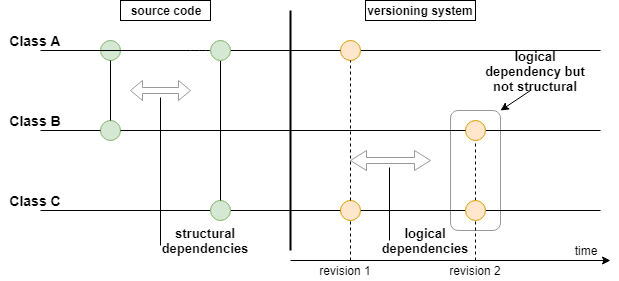
\includegraphics[scale=0.43]{fig1.png}
\caption{Relationships between structural and logical dependencies }
\label{fig:fig1}
\centering
\end{figure}

Changes made to two modules in the same commit do not necessarily indicate the co-evolution of the two. These changes could be completely unrelated. The study \cite{Yu2007} acknowledges the fact that evolutionary coupling could also be determined accidentally by two modules changing in the same commit (independent evolution, as it is called) and this will bring noise to the measurement of logical coupling. 

In our work we investigate which are the patterns of repeated co-change that produce true logical dependencies. This paper is organized as follows: Section \ref{sec:state} discusses the state of the art regarding the detection and usage of logical dependencies. In Section \ref{sec:tool} we describe our tool used to analyze software systems in order to extract structural and logical dependencies. Section \ref{sec:results} presents our experimental results on a set of open source systems. Future work is outlined in Section \ref{sec:future}, while Section \ref{sec:conclusion} summarizes our concluding remarks.



\section{State of the art}
\label{sec:state}
The current software engineering trends recommend that general dependency management methods and tools should also include logical dependencies besides the structural dependencies that are extracted by analyzing the source code \cite{Oliva:2011:ISL:2067853.2068086}, \cite{DBLP:journals/jss/AjienkaC17}, \cite{Yu2007}. 

The concepts of logical coupling and logical dependencies were first used in different analysis tasks, all related to changes: for software change impact analysis \cite{1553643}, for identifying the potential ripple effects caused by software changes during software maintenance and evolution \cite{DBLP:conf/issre/OlivaG15}, \cite{Oliva:2011:ISL:2067853.2068086}, \cite{Poshyvanyk2009}, \cite{posh2010} or for their link to deffects \cite{wiese}, \cite{Zimmermann:2004:MVH:998675.999460}. But, in order to add logical dependencies besides structural dependencies as inputs for methods and tools for dependency management and analysis, co-changes must be filtered until they remain only a reduced but relevant set of true logical dependencies. 

There are researches that investigated quantitative aspects of logical dependencies and their interplay with structural dependencies. 
Oliva and Gerosa \cite{Oliva:2011:ISL:2067853.2068086}, \cite{DBLP:conf/issre/OlivaG15} have found first that the set of co-changed classes was much larger compared to the set of structurally coupled classes. They identified structural and logical dependencies from 150000 revisions from the Apache Software Foundation SVN repository. Also they concluded  that in at least 91\% of the cases, logical dependencies involve files that are not structurally related. This implies that not all of the change dependencies are related to structural dependencies and there could be other reasons for software artifacts to be change dependent.




Zimmermann et al \cite{Zimmermann:2004:MVH:998675.999460} introduced data mining techniques to obtain association
rules from version histories.
The mined association rules  have a probabilistic interpretation based on the amount of
evidence in the transactions they are derived from. This
amount of evidence is determined by two measures: 
support and confidence.  They developed a tool to predict future or
missing changes.



In order to add logical dependencies besides structural dependencies as inputs for methods and tools for dependency management and analysis, class co-changes must be filtered until they remain only a reduced but relevant set of true logical dependencies. 


\section{Tool for measuring software dependencies}
\label{sec:tool}



\begin{figure*}[htb]
\centering
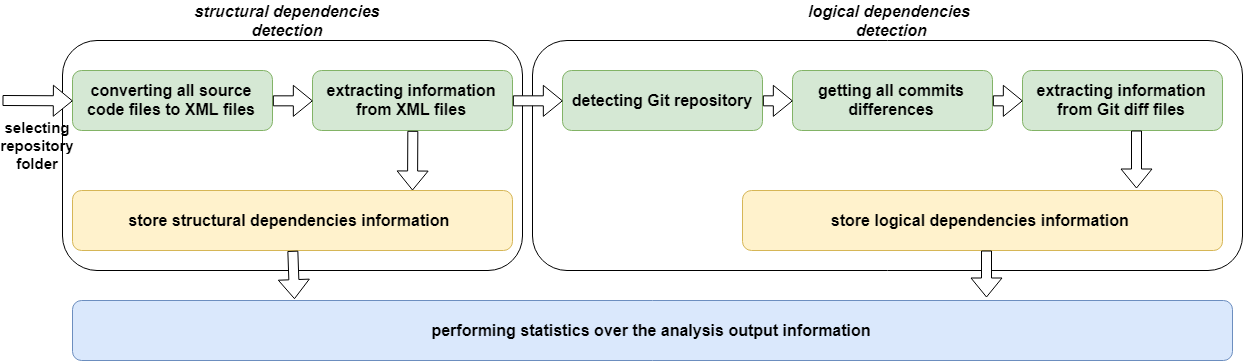
\includegraphics[width=\textwidth]{fig3.png}
\caption{Processing phases}
\label{fig:fig3}
\end{figure*}

In order to build structural and logical dependencies we have developed a tool that takes as input the source code repository and builds the required software dependencies. The workflow can be delimited by three major steps as it follows (Figure \ref{fig:fig3}):\\ \\
\textit{\textbf{Step 1:} Extracting structural dependencies.}\\
\textit{\textbf{Step 2:} Extracting logical dependencies.}\\
\textit{\textbf{Step 3:} Processing the information extracted.}


\subsection{ Extracting structural dependencies}

A structural dependency between two classes A and B is given by the fact that A statically depends on B, meaning that A cannot be compiled without knowing about B. In object oriented system, this dependency can be given by many types of relationships between the two classes: A extends B, A implements B, A has attributes of type B, A has methods which have type B in their signature, A uses local variables of type B, A calls methods of B.


 We use an external tool called srcML \cite{2003:XLC:851042.857028},
\cite{Collard:2011:LTF:2067850.2068011} to convert all source code files from the current release into XML files. All the information about classes, methods, calls to other classes are afterwards extracted by our tool parsing the XML files and building a dependencies data structure. We have chosen to rely on srcML as a preprocessing tool because it reduces a significant number of syntactic differences from different programming languages and can make easyer the parsing of source code written in different programming languages such as Java, C++ and C\#.    

\subsection{Extracting logical dependencies}

The versioning system contains the long-term change history of every file. Each project change made by an individual at a certain point of time is contained into a commit \cite{svn}. All the commits are stored in the versioning system chronologically and each commit has a parent. The parent commit is the baseline from which development began, the only exception to this rule is the first commit which has no parent. We will take into consideration only \textit{commits that have a parent} since the first commit can include source code files that are already in development (migration from one versioning system to another) and this can introduce redundant logical links \cite{DBLP:journals/jss/AjienkaC17}. 

The tool looks through the main branch of the project and gets all the existing commits. For each commit a diff against the parent will be made and stored. Here we have the option to ignore commits that contain more files than a threshold value for commit size. Also, we have the option to check whether the differences are in actual code or if they affect only parts of source files that are only comments.  Finally after all the difference files are stored, all the files are parsed and logical dependencies are build. For a group of files that are committed together, logical dependencies are added between all pairs formed by members of the group. Adding a logical dependency increases an occurrence counter for the logical link. 

\section{Filtering mechanisms for logical dependencies and why we need them}
\label{sec:results}


We have analyzed a set of open-source projects found on GitHub\footnote{http://github.com/} \cite{Kalliamvakou2016} in order to extract the structural and logical dependencies between classes. Table \ref{table:1} enumerates all the systems studied. The 1st column assigns the projects IDs; 2nd column shows the project name; 3rd column shows the number of entities(classes and interfaces) extracted; 4th column shows the number of most recent commits analyzed from the active branch of each project and the 5th shows the language in which the project was developed.
\begin{table}[!h]
\renewcommand{\arraystretch}{1.25}
\caption{Summary of open source projects studied.}
\label{table:1}
\centering
\begin{tabular}{|c|c|c|c|c|c|}
\hline
   ID  & Project    & Nr. of & Nr. of& Type\\
     &     & entites & commits & \\
\hline
1	&	bluecove	&	586	&	894	&	java	\\
2	&	aima-java	&	987	&	818	&	java	\\
3	&	powermock	&	1084	&	893	&	java	\\
4	&	restfb	&	783	&	1188	&	java	\\
5	&	rxjava	&	2673	&	2468	&	java	\\
6	&	metro-jax-ws	&	1103	&	2222	&	java	\\
7	&	mockito	&	1409	&	1572	&	java	\\
8	&	grizzly	&	1592	&	3122	&	java	\\
9	&	shipkit	&	242	&	1483	&	java	\\
10	&	OpenClinica	&	1653	&	3749	&	java	\\
11	&	robolectric	&	2050	&	5029	&	java	\\
12	&	aeron	&	541	&	5101	&	java	\\
13	&	antlr4	&	1381	&	3449	&	java	\\
14	&	mcidasv	&	805	&	3668	&	java	\\
15	&	ShareX	&	919	&	2505	&	csharp	\\
16	&	aspnetboilerplate	&	2353	&	1615	&	csharp	\\
17	&	orleans	&	3485	&	3353	&	csharp	\\
18	&	cli	&	767	&	2397	&	csharp	\\
19	&	cake	&	2250	&	1853	&	csharp	\\
20	&	Avalonia	&	1677	&	2445	&	csharp	\\
21	&	EntityFramework	&	7107	&	2443	&	csharp	\\
22	&	jellyfin	&	2179	&	4065	&	csharp	\\
23	&	PowerShell	&	861	&	2033	&	csharp	\\
24	&	WeiXinMPSDK	&	2029	&	2723	&	csharp	\\
25	&	ArchiSteamFarm	&	117	&	2181	&	csharp	\\
26	&	VisualStudio	&	1016	&	4417	&	csharp	\\
27	&	CppSharp	&	259	&	3882	&	csharp	\\
\hline
\end{tabular}
\end{table}

\subsection{Estimating the number of co-changing classes vs the number of structural dependencies}
\label{sec:preliminary}

In a preliminary experiment, we consider every pair of classes that change together in any transaction  as a logical dependency. By extracting all the logical dependencies(LD) of all systems from table \ref{table:1} and comparing  their number with the number of structural dependencies,  we found that, in average for a system,  the logical dependencies outnumber the structural dependencies by an average factor of 300.  

It is clear that we cannot use the extracted logical dependencies(LD) obtained from all pairs of co-changing classes, since their number is much too high and we have to find filtering mechanisms in order to reduce their number until it becomes comparable or smaller than the number structural dependencies(SD), and there remain only the most significant, valid logical dependencies.
In the following subsections we will define two filtering mechanisms for logical dependencies.

\subsection{Filtering based on commit transaction size}

We define the size of a commit transaction (cs) as the total number of source code files that have changed. Big commit transactions can be due to merges with other branches or folders renamings. In this case, a series of irrelevant logical dependencies can be introduced since not all the files are updated in the same time for a development reason. Different related works ignore logical dependencies produced by big commit transactions, by choosing fixed threshold values for the maximum number of files accepted in a commit transaction \cite{DBLP:journals/jss/AjienkaC17}, \cite{DBLP:journals/ese/AjienkaCC18}, \cite{Beck:2011:CMC:2025113.2025162}.


Before we decided to also put a fixed threshold over the size of commit transactions we analyzed the overall transaction size trend of our studied the systems.
In order to do this we have chosen the following threshold values for the number of files in a commit transaction: 5, 10, 20 and no threshold (infinity) and we counted the number of commit transactions that fall into each category.


\begin{figure}[h]
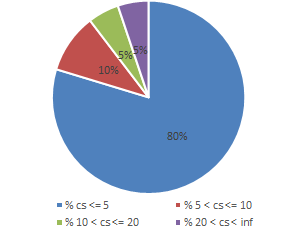
\includegraphics[scale=0.9]{fig_cs.png}
\caption{Commit transaction size(cs) trend in percentages}
\label{fig:fig_cs}
\centering
\end{figure}


Based on the results presented in Figure \ref{fig:fig_cs} we can say that 90\% of the total commit transactions made are with less than 10 source code files changed. This percent allows us to say that setting a threshold of 10 files for the maximum size of the commit transactions will not affect so much the total number of commit transactions from the systems since it will still remain 90\% of the commit transactions from where we can extract logical dependencies.


\begin{figure}[h]
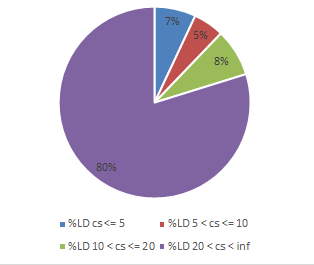
\includegraphics[scale=0.9]{fig_ld_ts.png}
\caption{Percentages of LD extracted from each commit transaction size(cs) group}
\label{fig:fig_ld_ts}
\centering
\end{figure}

So, how will this threshold will help in filtering the huge amount of extracted logical dependencies from the systems?
As we can see in Figure \ref{fig:fig_ld_ts} even though only 5\% of the commit transactions have more than 20 files changed ($20<cs<inf$) they generate in average 80\% of the total amount of logical dependencies extracted from the systems.
The high number of logical dependencies extracted from such a small number of commit transactions is caused by big commit transactions. 
One single big commit transaction can lead to a large amount of logical dependencies. For example in RxJava we have a very few commit transactions with 1030 source code files, this means that those files can generate 
$\Comb{n}{k}=\frac{n!}{k!(n-k)!} = \frac{1030!}{2!(1028)!} = 529 935$ logical dependencies. By setting a threshold on the commit transaction size we can avoid the introduction of those logical dependencies into the system.

So filtering 10\% of the total amount of commit transactions can indeed lead to a significant decrease of the amount of logical dependencies and that is why we choose the value of 10 files as our fixed threshold for the maximum size of a commit transaction.

We computed again the number of logical dependencies from all the test systems, and found out that, in average for a system, it outnumbers the structural dependencies by an average factor of 9.  Compared with the average factor of 300 determined in the conditions of subsection \ref{sec:preliminary}, it is a very significant improvement.


\subsection{Filtering based on the number of occurrences}
\label{sec:filterocc}
Filtering only based on the commit transaction size is not enough to filter logical dependencies since the remaining amount still exceeds the amount of structural dependencies by an average factor of 9 which is still too big. 
One occurrence of a co-change between two entities cannot be a valid logical dependency since that can be a coincidence. If two entities have multiple occurrences of co-changes then the probability of a coincidence is smaller. We define a threshold value for the minimum number of occurrences (occ) of a co-change in order to be considered a valid logical dependency.
We have performed a series of analysis on the test systems, incrementing the threshold value occ from 1 to 4. In each of the cases the extracted logical dependencies from commit transaction with less or equal to 10 changed source code files were also filtered by the minimum number of occurrences established and all the logical dependencies that did not exceeded the minimum number of occurrences were discarded. 

The results of the analysis are presented in Table \ref{table:sd_percentages} as percentages of logical dependencies (LD) that are also structural dependencies and Table \ref{table:ld_ratio} as ratio of the number of logical dependencies (LD) to the number of structural dependencies (SD).



\begin{table}[!h]
\renewcommand{\arraystretch}{1.25}
\caption{Percentage of LD that are also SD}
\label{table:sd_percentages}
\centering
\begin{tabular}{|c|c|c|c|c|}
\hline
    ID  & $occ\geq 1$ & $occ\geq 2$ & $occ\geq 3$ & $occ\geq 4$  \\
\hline
1	&	1,56	&	1,99	&	1,88	&	6,96	\\
2	&	8,32	&	10,60	&	11,74	&	11,89	\\
3	&	1,99	&	2,41	&	3,14	&	5,46	\\
4	&	0,54	&	0,60	&	0,47	&	0,44	\\
5	&	1,29	&	1,41	&	2,40	&	2,34	\\
6	&	5,18	&	7,00	&	7,64	&	6,79	\\
7	&	2,56	&	2,89	&	4,83	&	5,06	\\
8	&	3,11	&	4,75	&	6,98	&	7,50	\\
9	&	5,23	&	7,58	&	9,44	&	10,07	\\
10	&	5,05	&	5,10	&	6,43	&	6,30	\\
11	&	1,82	&	2,57	&	3,32	&	4,11	\\
12	&	6,67	&	8,97	&	9,60	&	10,43	\\
13	&	0,72	&	1,59	&	2,65	&	2,30	\\
14	&	5,49	&	8,52	&	8,40	&	8,36	\\
15	&	4,02	&	6,35	&	7,03	&	8,63	\\
16	&	5,00	&	6,83	&	6,85	&	6,65	\\
17	&	2,41	&	2,59	&	2,89	&	2,99	\\
18	&	3,03	&	3,90	&	5,06	&	6,71	\\
19	&	1,72	&	2,17	&	1,51	&	1,25	\\
20	&	4,44	&	6,20	&	6,73	&	7,54	\\
21	&	1,22	&	2,18	&	2,47	&	2,07	\\
22	&	2,55	&	3,31	&	4,17	&	4,67	\\
23	&	3,95	&	6,57	&	8,25	&	9,38	\\
24	&	1,84	&	3,00	&	4,03	&	5,03	\\
25	&	0,42	&	0,59	&	0,73	&	0,77	\\
26	&	1,01	&	1,50	&	1,82	&	2,11	\\
27	&	3,87	&	5,05	&	5,59	&	5,86	\\

\hline
Average	&	2,56	&	3,15	&	4,50	&	5,88	\\


\hline
\end{tabular}
\end{table}


\begin{table}[!h]
\renewcommand{\arraystretch}{1.25}
\caption{Ratio of number of LD to number of SD}
\label{table:ld_ratio}
\centering
\begin{tabular}{|c|c|c|c|c|}
\hline
    ID  & $occ\geq 1$ & $occ\geq 2$ & $occ\geq 3$ & $occ\geq 4$  \\
\hline
1	&	15,64	&	7,36	&	4,65	&	0,99	\\
2	&	1,80	&	0,73	&	0,35	&	0,23	\\
3	&	16,10	&	6,10	&	2,45	&	1,18	\\
4	&	121,01	&	95,24	&	86,90	&	82,32	\\
5	&	12,66	&	8,60	&	2,63	&	2,17	\\
6	&	2,78	&	1,20	&	0,79	&	0,60	\\
7	&	11,88	&	6,73	&	2,81	&	2,04	\\
8	&	9,40	&	3,65	&	1,75	&	1,14	\\
9	&	11,55	&	6,45	&	3,61	&	2,46	\\
10	&	2,87	&	2,04	&	0,96	&	0,70	\\
11	&	24,84	&	14,02	&	9,20	&	6,38	\\
12	&	8,22	&	4,52	&	3,09	&	2,23	\\
13	&	27,09	&	8,47	&	3,26	&	2,74	\\
14	&	7,23	&	3,61	&	2,74	&	2,28	\\
15	&	8,08	&	3,12	&	1,91	&	1,03	\\
16	&	3,63	&	1,41	&	0,76	&	0,54	\\
17	&	6,94	&	4,08	&	2,27	&	1,63	\\
18	&	6,52	&	3,79	&	1,84	&	1,09	\\
19	&	12,40	&	7,38	&	3,90	&	3,41	\\
20	&	3,85	&	1,85	&	1,19	&	0,69	\\
21	&	14,79	&	4,95	&	2,91	&	2,20	\\
22	&	7,57	&	4,24	&	2,21	&	1,65	\\
23	&	8,68	&	3,04	&	1,89	&	1,06	\\
24	&	9,20	&	4,35	&	2,41	&	1,64	\\
25	&	41,46	&	30,04	&	23,98	&	21,44	\\
26	&	10,45	&	5,47	&	3,78	&	2,90	\\
27	&	14,42	&	8,04	&	5,55	&	4,20	\\

\hline
Average	&	9,30	&	4,44	&	2,54	&	1,64	\\

\hline
\end{tabular}
\end{table}




Based on Table \ref{table:sd_percentages} we can say that only a small percentage of the extracted logical dependencies are also structural dependencies. This is consistent with the findings of related works \cite{DBLP:journals/jss/AjienkaC17}, \cite{DBLP:journals/ese/AjienkaCC18}. The percentage of LD which are also SD  increases with the minimum number of occurrences because the number of logical dependencies from the systems decreases with the minimum number of occurrences. 
We calculate the overlapping between logical and structural dependencies not only because we want to get an idea of how many structural dependencies are reflected in the versioning system through logical dependencies but also because we want to eliminate logical dependencies that are also structural dependencies since they don't bring any new information to the systems.

We stopped the minimum occurrences threshold to 4 because we observed that for systems with ID 2, 6, 10 and 16 from Table \ref{table:ld_ratio} the ratio number is lower than 1 which means that the number of SD is higher than the number of LD. On the other hand for systems with ID 4, 11, 19, 25 the threshold of 4 for minimum number of occurrences does not change the discrepancy between the number of logical and structural dependencies.
If we try to go higher with the occurrences threshold we will risk to filter all the existing logical dependencies for some of the systems.
So, filtering with a threshold of 4 for the minimum number of occurrences will indeed filter the logical dependencies but for some of the systems the remaining number of logical dependencies will still be significantly higher compared to the number of structural dependencies.



\section{Future work}
\label{sec:future}
As we could see in section \ref{sec:filterocc} filtering logical dependencies based on a fixed value threshold for the number of occurrences achieves a degree of filtering which is satisfactory in average: when $occ\geq 4$ the number of logical dependencies is comparable with the number of logical structural dependencies. However, as it results from the detailed situation presented in Table \ref{table:ld_ratio}, this kind of filtering is not always the best solution for each test system.
The threshold for occurrences may also be related to the number of commits of the system. Logical dependencies from systems with 5000 commits will have more chances to occur than logical dependencies from systems with 1000 commits. Also the number of entities from the systems can influence the number of occurrences. A system with a small number of entities and a big number of commits may have bigger numbers of occurrences since there are not so many combinations of entities that can appear together.
We will try to establish all the factors that influence the number of occurrences and dynamically calculate the threshold value for the minimum number of occurrences for each system.

Also, we consider that in the future, the validation of extracted logical dependencies will occur by using them to enhance dependency graphs for applications such as architectural reconstruction \cite{Shtern:2012:CMS:2332427.2332428}, \cite{sar}  through clustering \cite{SoraConti} or finding of key classes \cite{PagerankENASE}, and evaluating the positive impact on their results.


\section{Conclusion}
\label{sec:conclusion}
In this work we experimentally define methods to filter out the most relevant logical dependencies from co-changing classes. 

Our experiments identified two important factors which affect the quality of logical dependencies are: the maximum number of files allowed in a commit transaction to be counted as logical dependency, and the minimum number of repeated occurrences for a co-change to be counted as logical dependency.

%\section*{References}

\bibliographystyle{IEEEtran}
% argument is your BibTeX string definitions and bibliography database(s)
\bibliography{IEEEabrv,logicaldepd}

\end{document}
